\section*{\begin{tabular*}{\linewidth}{@{}l @{\extracolsep{\fill}} r@{}}
Nr.~10 & PIK~87/3 \\
\end{tabular*} 
}

\textsf{\textbf{Pikunda (\mbox{Sangha}, Fpl.~255)}}

\vspace{1em}

\noindent\begin{tabular}{@{}rl@{}}
	\textbf{Feldarbeit:} & \begin{tabular}[t]{@{}l@{}}\textbf{03.06.--07.06.1987}\\ \textbf{(C. Kanimba Misago)}\end{tabular} \\ 
	\textbf{Abb.:} & \textbf{\ref{fig:PIK87-3_Skizze}--\ref{fig:PIK87-3_Funde}} \\ 
	\textbf{Tab.:} & \textbf{\ref{tab:PIK87-3_Funde}--\ref{tab:PIK87-3_14C-Daten}}\\
	\textbf{Taf.:} & \textbf{49.16--49.18} \\ 
	\textbf{Lit.:} & \textbf{\textsc{Kanimba Misago}~1995} \\ 
\end{tabular} 

\paragraph{Grabung und Befunde}\hspace{-.5em}|\hspace{.5em}%
Neben den beiden jeweils Grubenbefunden gewidmeten Grabungen PIK~87/1 und PIK~87/2 (Kat.-Nr.~8--9) wurde in Pikunda auch ein offener Ofen mit seitlichem, in eine Grube führenden Schlackenabfluss vom Typ \textit{Bamanya} untersucht \parencite[sieh][3235--3237]{Eggert.1987}.\footnote{Zur Praxis der Verhüttung in offenen Öfen mit seitlichem Schlackenabfluss siehe \textcites{vanNoten.1974}{Celis.1987}[38--46]{Celis.1991}{Ackerman.1999}.} Für diesen Befund liegen weder die schriftliche noch eine gezeichnete Dokumentation des Ausgräbers C. Kanimba Misago vor. Die einzigen schriftlichen Quellen sind der Auszug eines unpublizierten Manuskriptes des Ausgräbers, welches den Befund auf weniger als einer maschinengeschriebenen Seite knapp charakterisiert (\textsc{Kanimba Misago} 1995), sowie Notizen aus dem Feldbuch des Projektleiters M.~K.~H. Eggert. Es können keine Angaben darüber gemacht werden, wo in Pikunda sich der Befund in Relation zu den anderen ausgegrabenen Komplexen befand, da keine Einmessung erfolgte. Auf Basis einiger Übersichtsfotos lässt sich die Grabungssituation lediglich in einer groben Skizze rekonstruieren (Abb.~\ref{fig:PIK87-3_Skizze}). Der freigelegte Befund ist grundsätzlich in zwei Bereiche zu unterteilen: zum Einen die Ofenwanne beziehungsweise -plattform mit dem Schlackenabflusskanal und zum anderen die Schlackengrube.

\begin{figure*}[p]
 \centering
 \includegraphics[width=\textwidth]{fig/PIK87-3_Skizze.pdf}
 \caption{PIK~87/3: Überblicksskizze (auf Basis vorliegender Fotos).}
 \label{fig:PIK87-3_Skizze}
\end{figure*}

\begin{figure*}[p]
\centering
\begin{subfigure}[b]{.475\textwidth}
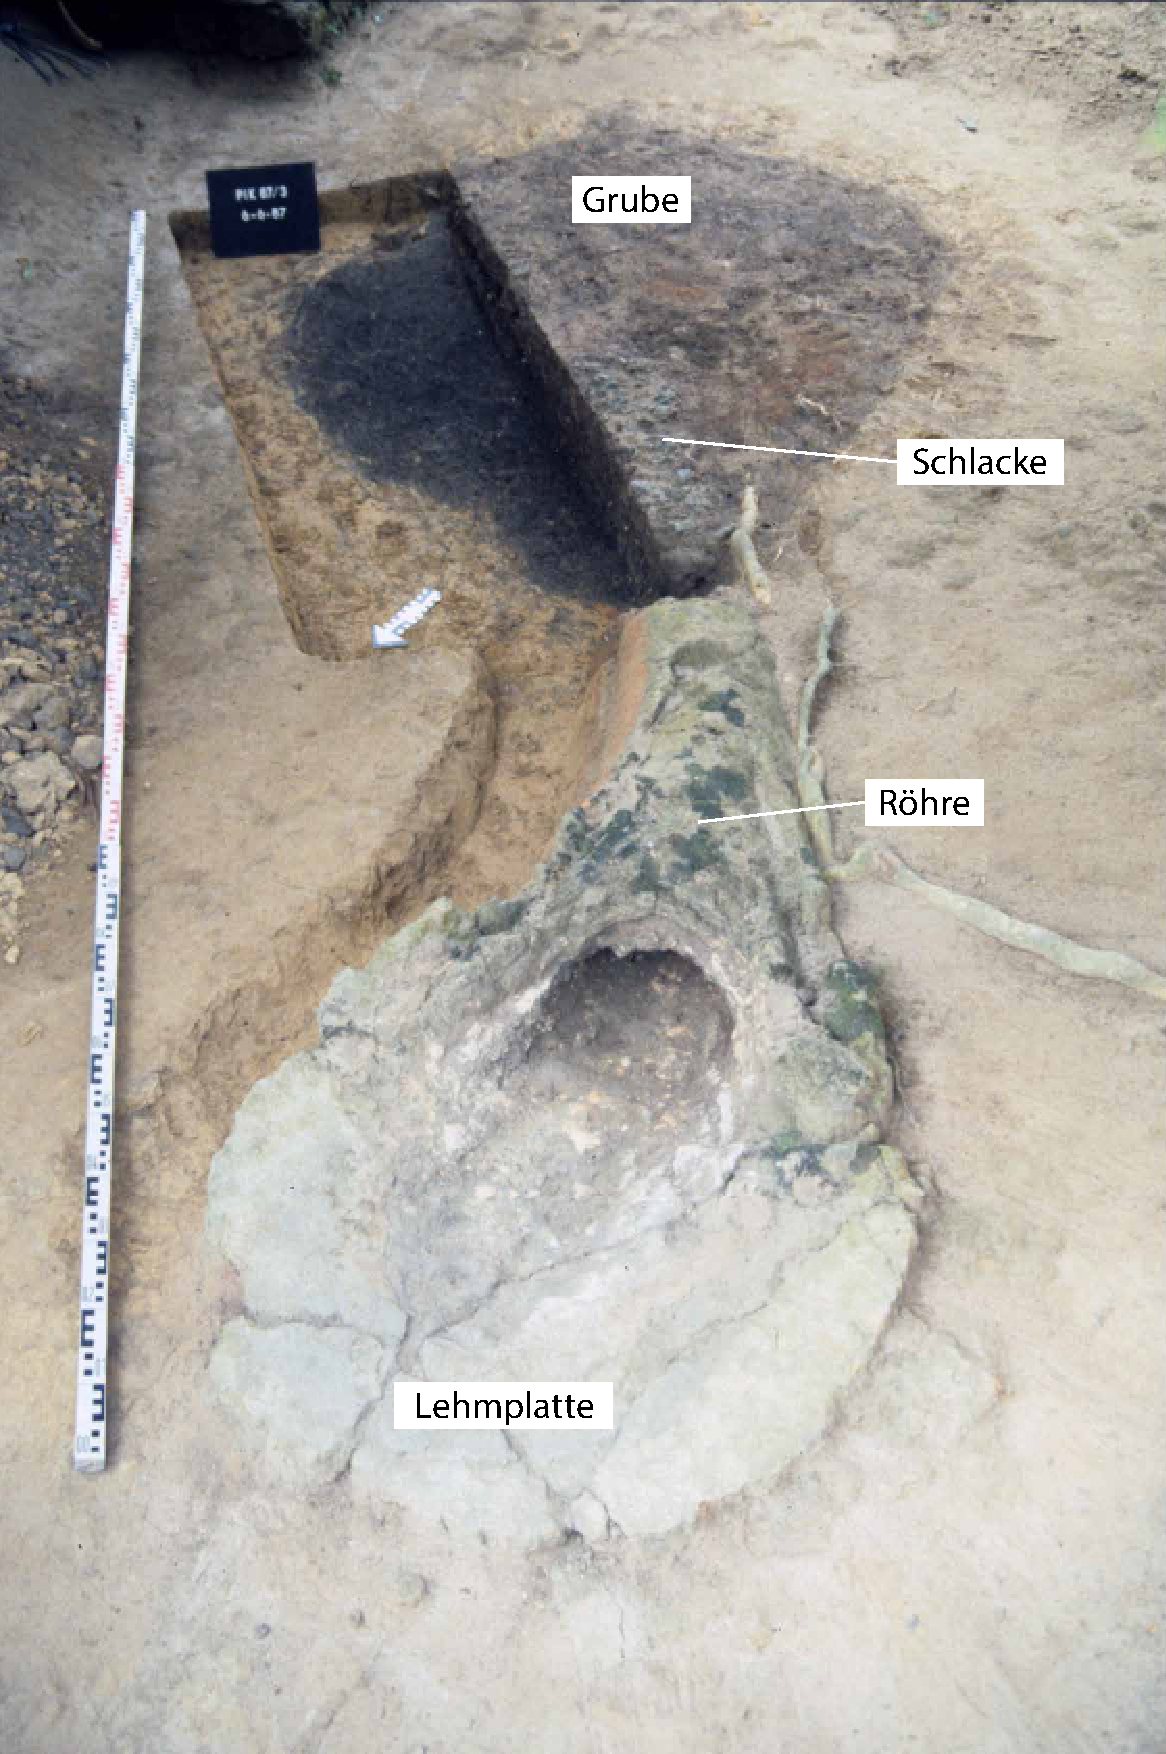
\includegraphics[width = \textwidth]{fig/PIK87-3_E87-016-20.pdf}
\caption{Blick von Nordwesten}
\label{fig:PIK87-3_vonNW}
\end{subfigure}\hfill
\begin{subfigure}[b]{.5015\textwidth}
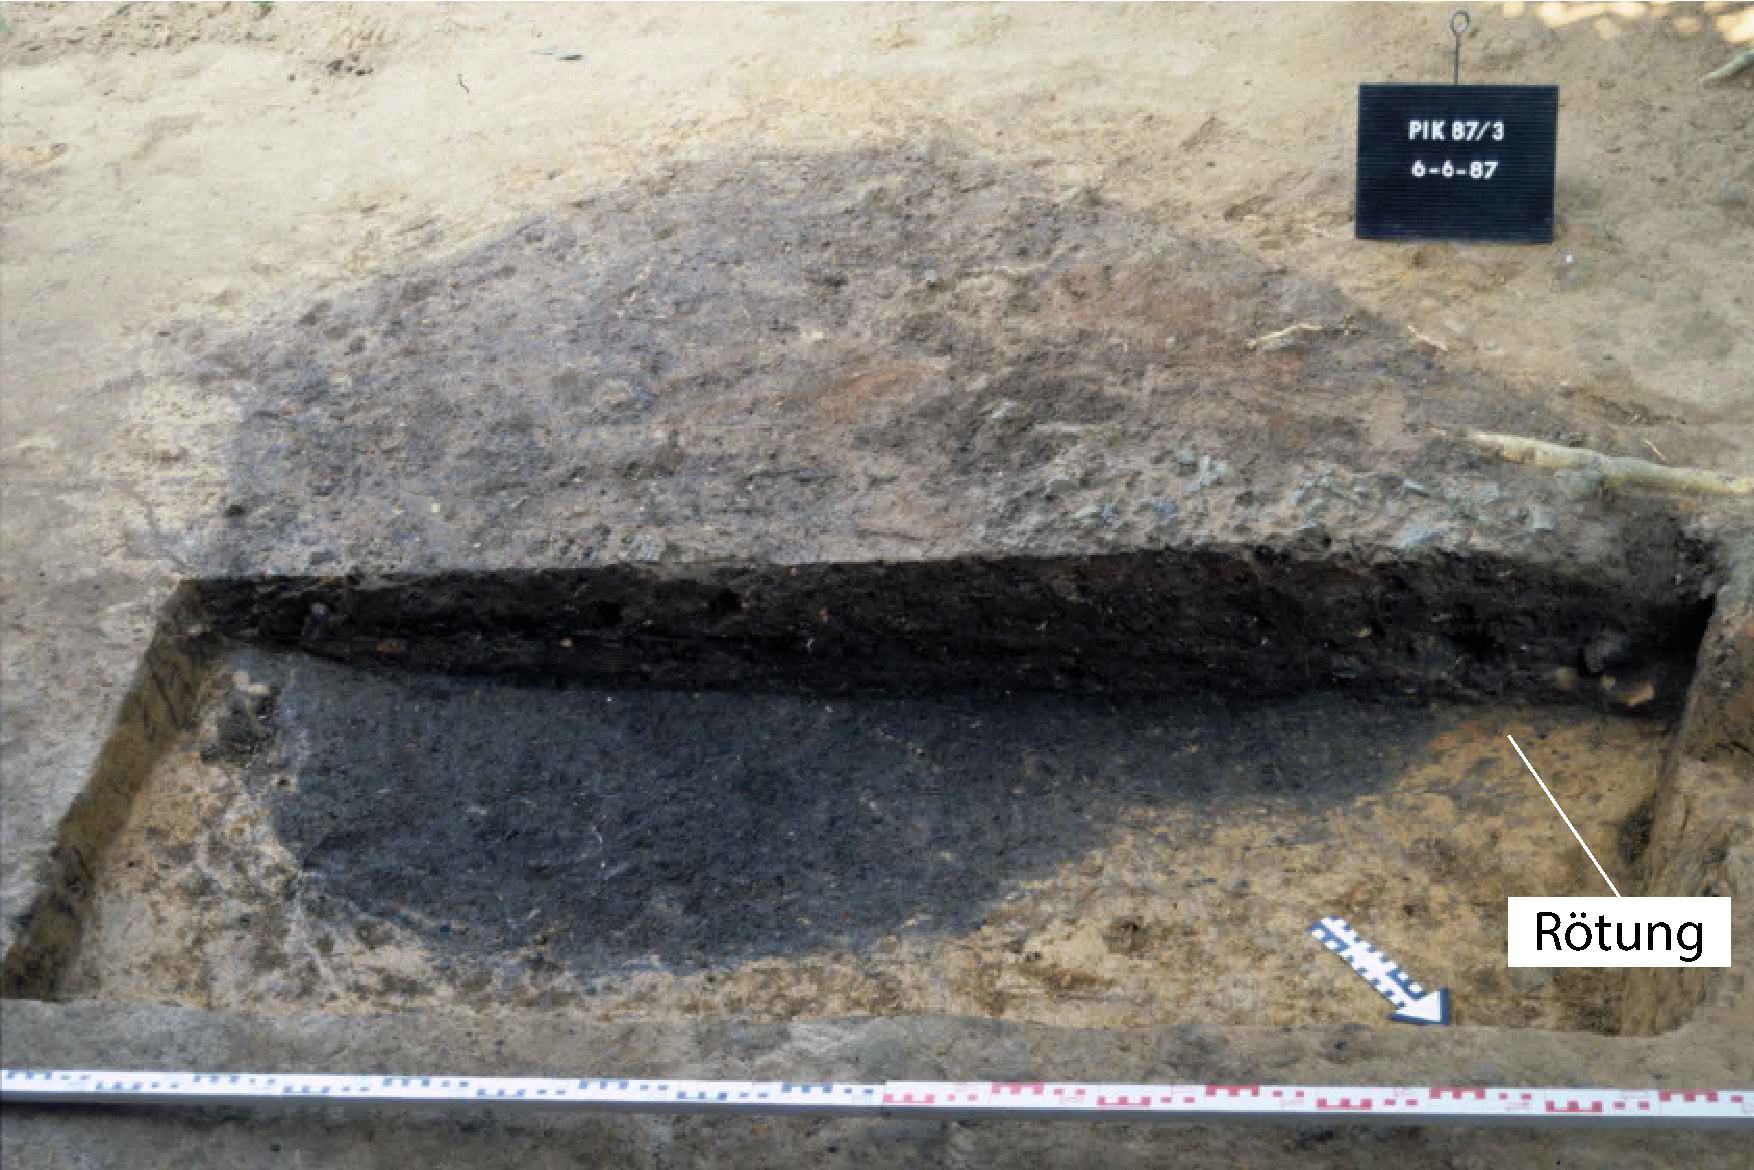
\includegraphics[width = \textwidth]{fig/PIK87-3_E87-016-24.pdf}
\caption{Grube von Nordosten}
\label{fig:PIK87-3_vonNO}
%\vspace{3ex}
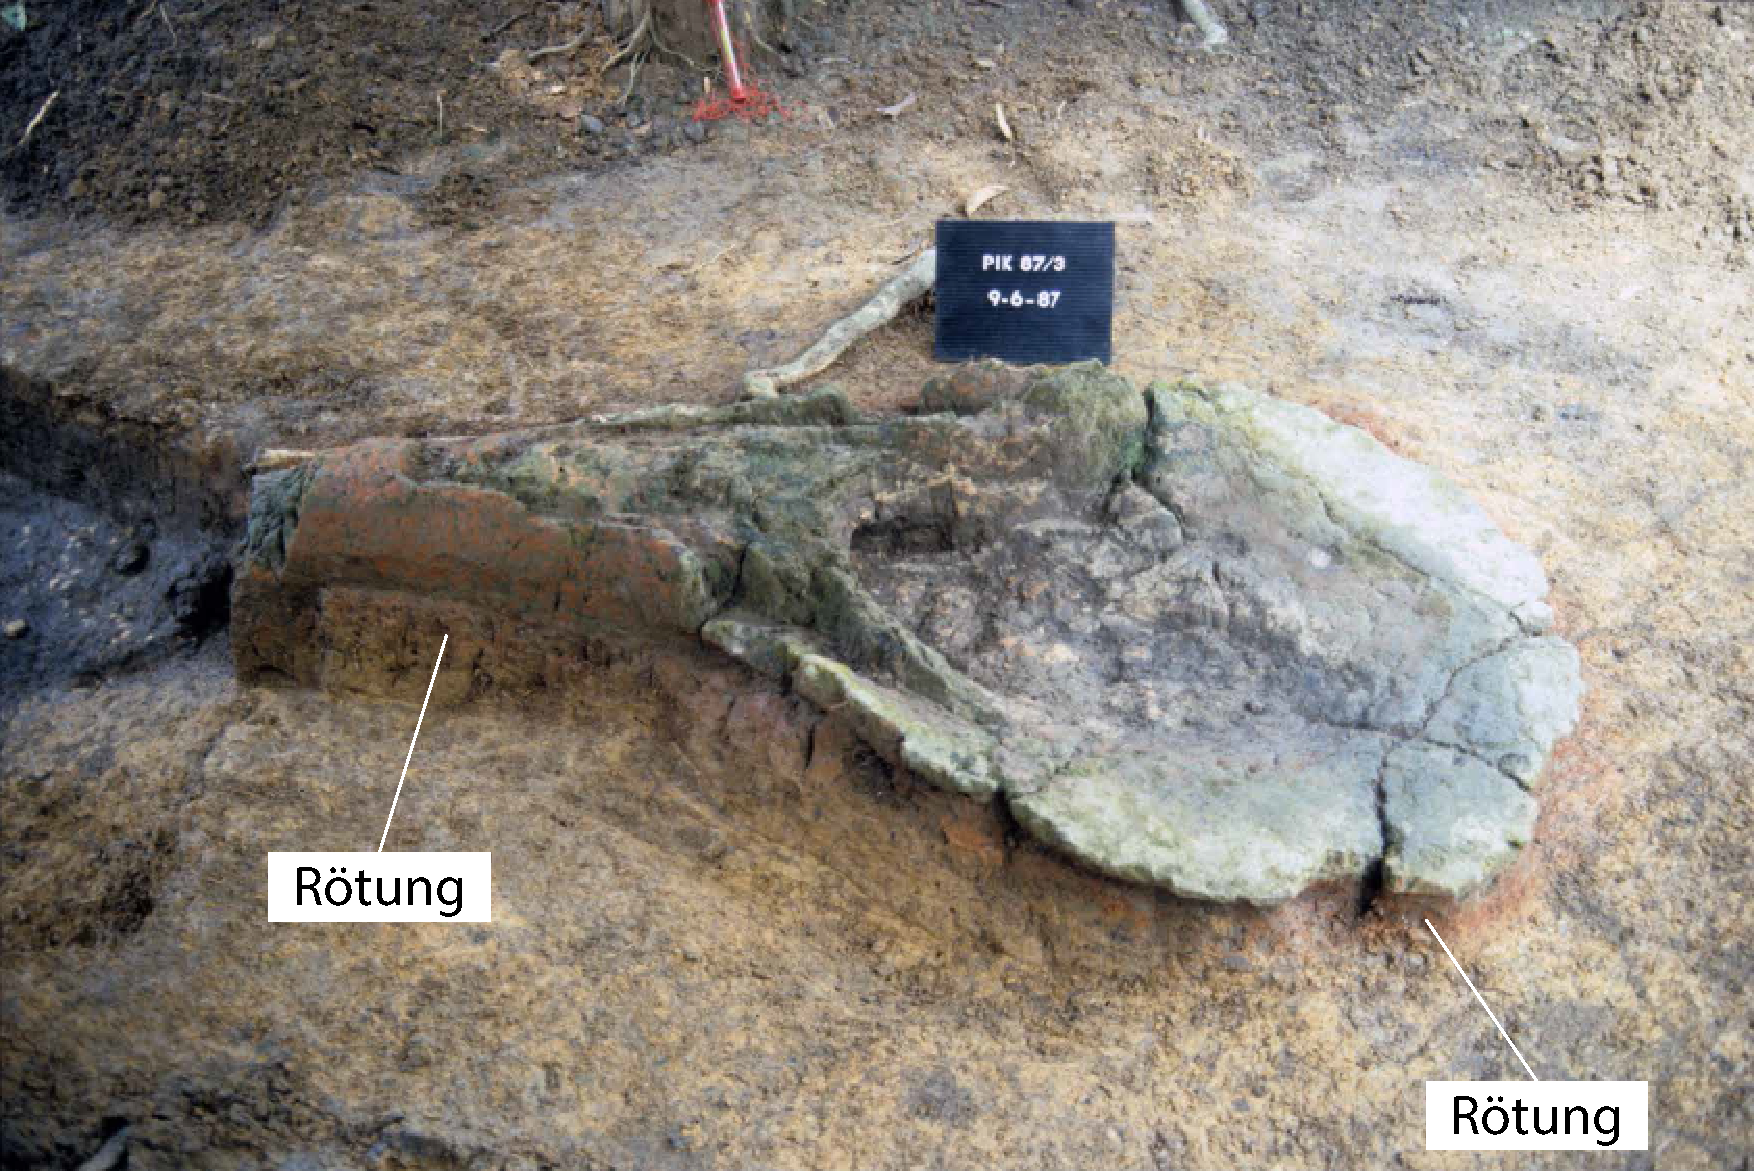
\includegraphics[width = \textwidth]{fig/PIK87-3_E87-019-2.pdf}
\caption{Lehmplatte von Osten}
\label{fig:PIK87-3_vonO}
\end{subfigure}
\caption{PIK~87/3: Situation am 06.06.1987 (A--B) und 09.06.1987 (C; Fotos: M.~K.~H.~Eggert).}
 \label{fig:PIK87-3_Fotos}
\end{figure*}

An der Oberfläche war der Befund durch eine leicht ovale, flache Lehmplatte zu erkennen, von der in südsüdöstlicher Richtung eine Fortsetzung -- der Schlackenabflusskanal -- zu einer Verfärbung führte (Abb.~\ref{fig:PIK87-3_vonNW}). Die etwa 7\,cm dicke Lehmplatte lag über dem Niveau der rezenten Oberfläche und ihr Rand sowie die obere Seite des Schlackenabflusskanals waren bereits deutlich von Erosion abgetragen (\textsc{Kanimba Misago} 1995). Sie hatte einen Durchmesser von zirka 1\,m. Nach dem Putzen der Oberfläche ließ sich eine etwa 10\,cm mächtige Rotverziegelung des anstehenden Sediments direkt unterhalb der Lehmplatte und entlang des Schlackenabflusskanals beobachten (Abb.~\ref{fig:PIK87-3_vonO}).

Der etwas über 1\,m lange Schlackenabflusskanal besteht aus demselben Material wie die Lehmplatte und geht direkt aus dieser hervor (Abb.~\ref{fig:PIK87-3_Fotos}). Er ist konisch geformt, Nordnordwest--Südsüdost-orientiert und in Richtung der Schlackengrube leicht geneigt. Die Wandungsdicke lag bei etwa 7\,cm (\textsc{Kanimba Misago} 1995) und die vorliegenden Fotos erwecken den Eindruck, dass die Wandung des Kanals aus zwei Lagen aufgebaut ist (Abb.~\ref{fig:PIK87-3_vonO}). Lehmplatte und Schlackenabflusskanal scheinen in einem Arbeitsgang hergestellt worden zu sein. Aufgrund der scharfen Grenzen zum umstehenden Lehm und der hellen Farbe handelt es sich mutmaßlich auch nicht um einen durch große Hitze \textit{in situ} verziegelten Befund, sondern eine aus Töpferton aufgebaute Struktur.

\begin{figure*}[!tb]
	\centering
	\begin{subfigure}[t]{0.32\textwidth}
		\centering
		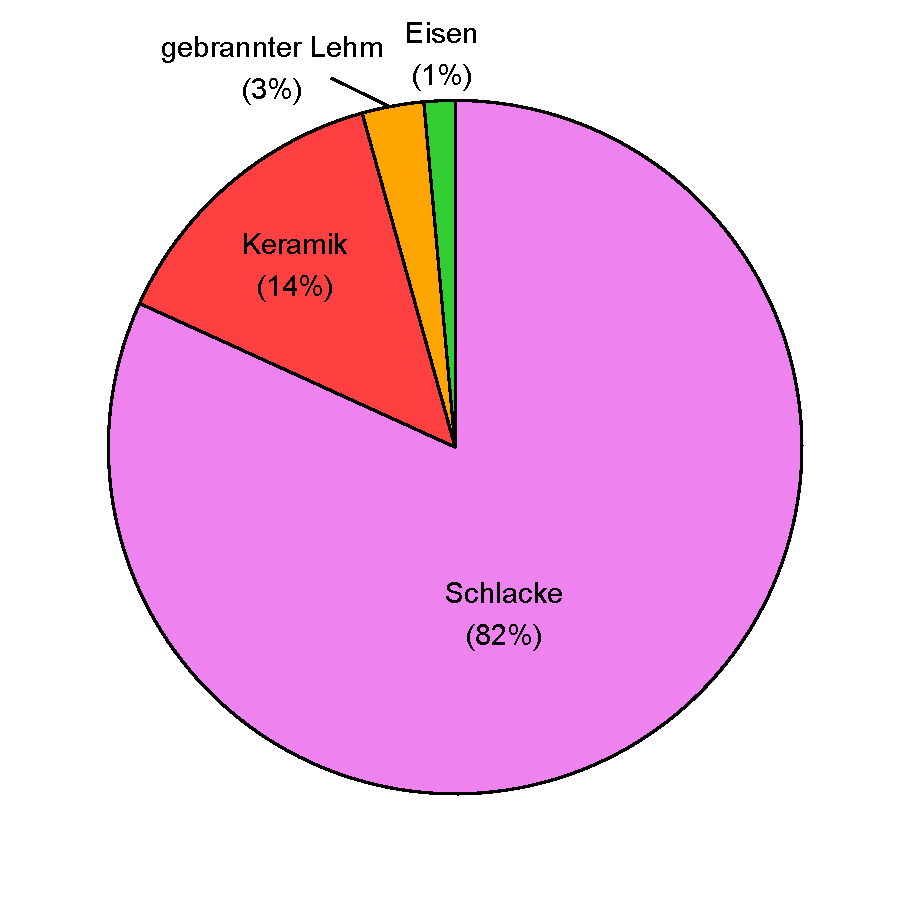
\includegraphics[width = \textwidth]{fig/9-10_PIK87-3_Funde_R_modDS.pdf}
		\caption{Funde.}
		\label{fig:PIK87-3_FundeArt}
	\end{subfigure}
	\begin{subfigure}[t]{0.32\textwidth}
		\centering
		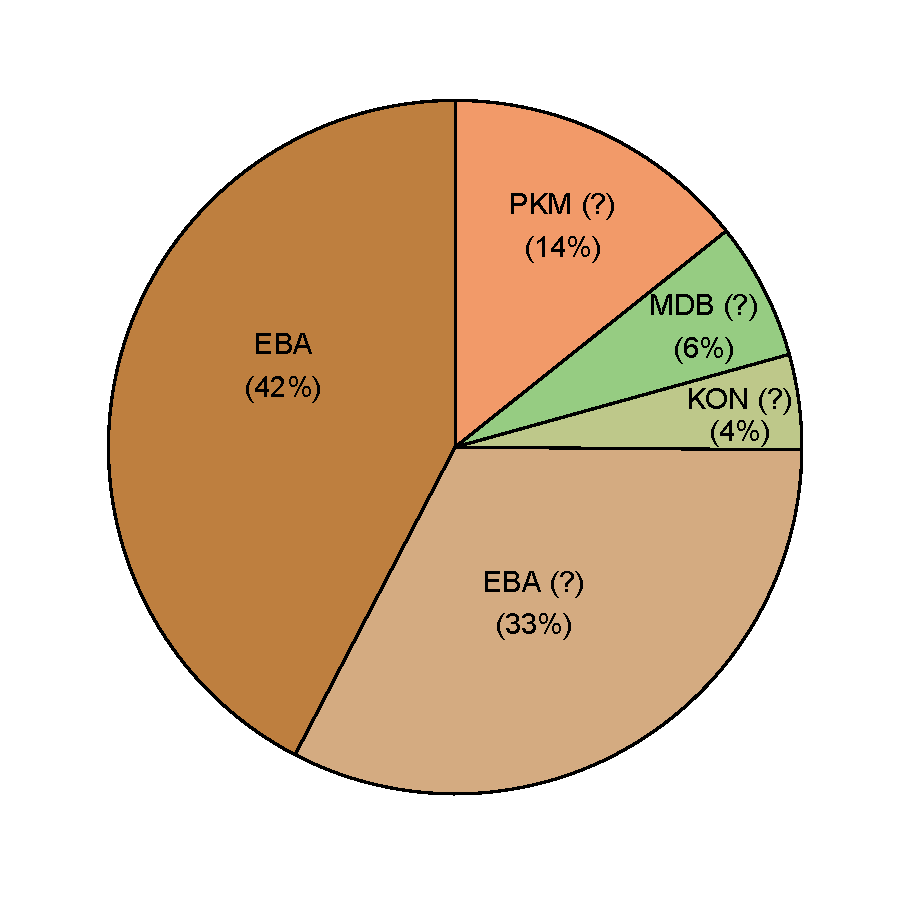
\includegraphics[width = \textwidth]{fig/9-10_PIK87-3_Stilgruppen_R_modDS.pdf}
		\caption{keramische Stilgruppen.}
		\label{fig:PIK87-3_Stilgruppen}
	\end{subfigure}
	\begin{subfigure}[t]{0.32\textwidth}
		\centering
		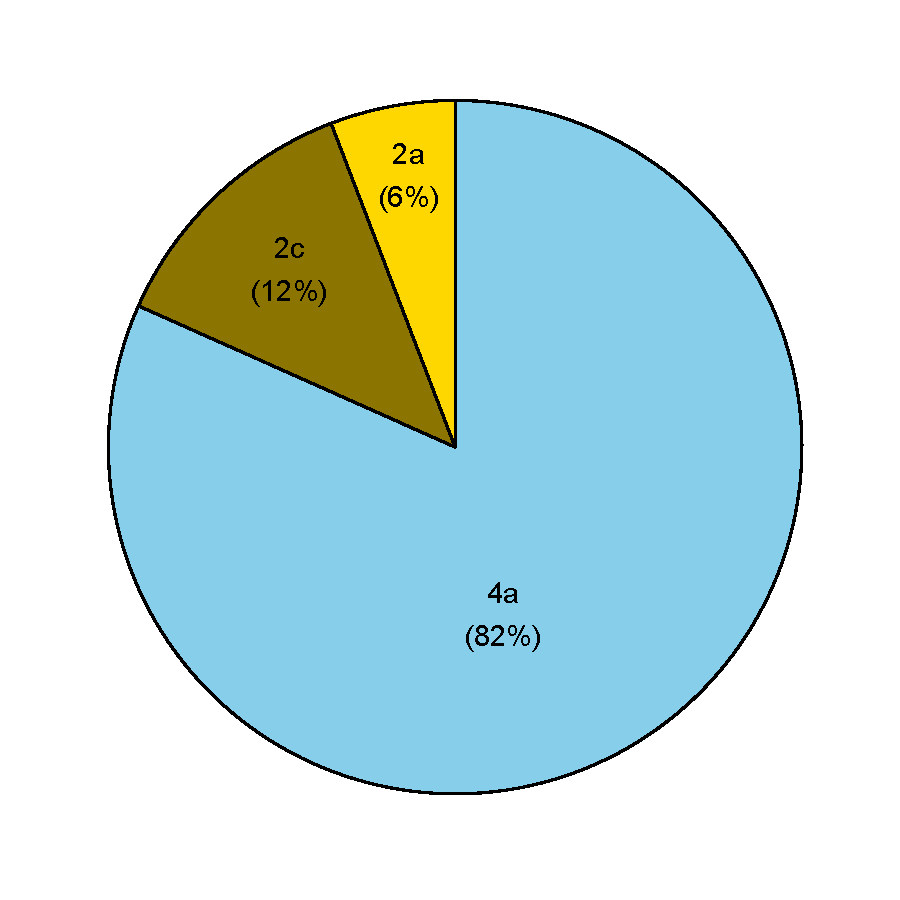
\includegraphics[width = \textwidth]{fig/9-10_PIK87-3_Schlacketypen_R_modDS.pdf}
		\caption{Schlacketypen.\vspace{1em}}
		\label{fig:PIK87-3_SchlackeTyp}
	\end{subfigure}
	\begin{subfigure}[t]{\textwidth}
		\centering
		\includegraphics[width = \textwidth]{fig/9-10_PIK87-3_Fragmentierung.pdf}
		\caption{Fragmentierung.}
		\label{fig:PIK87-3_Fragmentierung}
	\end{subfigure}
	\caption{PIK~87/3: Anteile der Fundmaterialien (A), keramischen Stilgruppen (B) und Schlacken (C) sowie Fragmentierungsgrad der Scherben (D; n~=~34; Größenklassen siehe Anm.~\ref{ftn:Keramik_Fragmentierung}).}
	\label{fig:PIK87-3_Funde}
\end{figure*}

\begin{table*}[!tb]	
	\centering
	{\footnotesize \begin{sftabular}{@{}lrrrr@{}}
\toprule
   \textbf{Fundkategorie} &  \textbf{Anzahl} &    \textbf{\%} &  \textbf{Gewicht (kg)} &    \textbf{\%} \\
\midrule
           Eisen &       1 &   1,6 &          0,04 &   1,4 \\
 gebrannter Lehm &       1 &   1,6 &          0,07 &   2,9 \\
         Keramik &      34 &  54,8 &          0,34 &  13,9 \\
        Schlacke &      26 &  41,9 &          1,99 &  81,8 \\
\bottomrule
\end{sftabular}
}
	\caption{PIK~87/3: Anteil verschiedener Fundmaterialien.}
	\label{tab:PIK87-3_Funde}
\end{table*}

Die südöstlich anschließende, etwa 1,5\,$\times$\,1\,m große Grube war als dunkle Verfärbung und durch eine leichte Fundstreuung bereits an der Oberfläche sichtbar. Für die Untersuchung dieser Grube wurde eine vom Ausgang des Schlackenabflusses ausgehende, Südost--Nordwest-orientierte Profilachse angelegt (Abb.~\ref{fig:PIK87-3_Skizze}, \ref{fig:PIK87-3_vonNW}--B). Der ursprünglich ausgegrabene Kasten A wurde relativ schnell um einen direkt anschließenden Kasten B erweitert, wodurch ein kompletter Profilschnitt durch die Grube entstand. Die beiden Schnittkästen waren zusammen etwa 1,8\,m breit. Im Bereich des Schlackenausflusses wurde die Grabungsfläche um eine dreieckige Fläche nach Nordwesten erweitert (Abb.~\ref{fig:PIK87-3_Skizze}).

Die Tiefe der Grube ist unklar, da keine Unterlagen vorliegen und auf keinem der Fotos ein vollständiges Profil zu sehen ist. \textsc{Kanimba Misago} (1995) berichtet, dass die Grube bis zur Sohle ausgegraben wurde, gibt jedoch keine Tiefe an. Alle vorhandenen Fotografien zeigen ausschließlich ein erstes Planum, das zirka 0,1--0,15\,m unter der Oberfläche liegt (Abb.~\ref{fig:PIK87-3_vonNW}--B). Die Befundgrenzen sind scharf und die unter der Lehmplatte und dem Schlackenausflusskanal beobachtete Verziegelung des anstehenden Lehms findet sich auch im unmittelbar an den Schlackenausflusskanal angrenztenden Bereich der Grube.

\begin{table*}[tb!]
	\centering
	{\footnotesize
		\begin{sftabular}{@{}llllr@{}}
			\toprule 
			\textbf{Lab-Nr} & \textbf{Datum (bp)} & \textbf{Datum (2-Sigma)} & \textbf{Probe} & \textbf{Tiefe} \\ 
			\midrule 
			KI-2892 & 840\( \pm \)41 & \begin{tabular}[t]{@{}l@{}}1048--1085 n.~Chr. (7,8\,\%);\\ 1124--1138 n.~Chr. (2\,\%);\\ 1150--1270 n.~Chr. (85.7\,\%)\end{tabular} & 3 & 0,25\,m \\ 
			\bottomrule 
	\end{sftabular}}
	\caption{PIK 87/3: \textsuperscript{14}C-Datierung.}
	\label{tab:PIK87-3_14C-Daten}
\end{table*}

\paragraph{Keramik\vspace{.5em}}\mbox{}\\
\begin{tabular}{@{}lrl@{}}
Ausgesondert: & 80\,g & \\ 
Bearbeitet: & 257\,g & (76\,\%) \\ 
Insgesamt: & 337\,g & \\ 
\end{tabular} 

\vspace{1em}
\noindent Das Fehlen der Grabungsdokumentation erschwert auch die Einschätzung und Auswertung des Fundmaterials. So muss offenbleiben, ob das vorliegende Material sämtliche bei der Grabung angefallen Funde umfasst oder ob Stücke verworfen worden, wie dies bei den Inventaren der anderen beiden Grabungen in Pikunda geschah (Kat.-Nr.~8--9). Aus dem Verhüttungsbefund PIK~87/3 liegen insgesamt nur sehr wenige Funde vor. Das keramische Fundgut umfasst lediglich 337\,g beziehungsweise 34 Scherben, die wiederum lediglich 19~GE repräsentieren. Ein großer Teil des Materials konnte keiner keramischen Stilgruppe zugewiesen werden und eine zweifelsfreie formale Ansprache war nur im Fall einer GE möglich (Taf.~49.16). Es handelt sich um eine Wandungsscherbe, die den für die Gefäße der Ebambe-Gruppe (Kap.~\ref{sec:EBA-Gr}) typischen Kegelhals und schmalen Schulterabsatz aufweist. Der Schulterbereich ist mit horizontalen Bändern aus Rillen, Winkel- und Wellen- sowie Kreuzmustern und diagonalem Schachbrett verziert, während der Ansatz des Gefäßbauches mit \textit{banfwa-nfwa} verziert ist. Das Stück lässt sich morphologisch und ornamental sehr gut in das Spektrum der Ebambe-Gruppe einpassen, weist jedoch auffällig hohe Anteile nicht-plastischer Partikel im Scherben auf. Dies ist keinesfalls typisch für Ebambe-Keramik und der Scherben erinnert mehr an die ebenfalls im Bereich des mittleren \mbox{Sangha} verbreitete Keramik der Kondo-Gruppe (Kap.~\ref{sec:KON-Gr}, Tab.~\ref{tab:Fabrics_StilGr_Pct}).

Weitere Scherben mit flächiger \textit{banfwa-nfwa}-Verzierung sind vorläufig ebenfalls Ebambe-Gruppe zugerechnet (Abb.~\ref{fig:PIK87-3_Funde}). Diese sowie die beschriebene GE machen 75\,\% des aus dem Befund stammenden, stilistisch ansprechbaren Keramik aus. Überdies fanden sich potentiell den Stilen Pikunda-Munda (Kap.~\ref{sec:PKM-Gr}), Mandombe (Kap.~\ref{sec:MDB-Gr}) und Konda (Kap.~\ref{sec:KON-Gr}) zuweisbare Scherben.\footnote{Potenziell der Konda-Keramik könnte das Randfragment einer kleinen Schale vom Typ I4 zugehörig sein, das eine Verzierung aus Rillen und Eindrücken auf dem Rand aufweist (Taf.~49.18).}

\paragraph{Sonstige Funde}\hspace{-.5em}|\hspace{.5em}%
Das Gros, etwa 82\,\% der knapp 2\,kg Schlacken lassen sich dem metallisch grauen, kantigen Typ 4a zuordnen (Abb.~\ref{fig:PIK87-3_SchlackeTyp}). Die restlichen 18\,\% sind Schlacken mit deutlichen Fließstrukturen des Typs 2a und 2c. Auffällig ist die teilweise stark rötlich bis violette Färbung einiger Schlackenstücke.\footnote{Zwei durch \textsc{Humphris \& Nordland} (2016) untersuchte Proben weisen auf eine Eisenproduktion bei nahezu optimalen Bedingungen hin. Um diese zu erzielen, ist nach \textsc{Humphris} und \textsc{Nordland} (ebd. 37) die Nutzung eines Flussmittels unerlässlich. In der Probe beobachtete hohe SiO$_{2}$-Anteile in Kombination mit den Daten einer ebenfalls untersuchten \textit{Tuyère} legen nahe, dass das Silizium-haltige Flussmittel aus einer Quarz-reichen technischen Keramik, zum Beispiel den \textit{Tuyères} freigesetzt wurde. Die grobe und Quarz-reiche Machart der untersuchten \textit{Tuyère} legt zudem eine solche Deutung des zugrundeliegenden Prozesse nahe, jedoch verbietet die unzureichende Anzahl untersuchter Proben von Schlacken sowie technischer Keramik eine klar umrissene Rekonstruktion. Eine Synthese aller Quellen zur Metallurgiegeschichte des nordwestlichen Kongobeckens ist im Rahmen einer gesonderten Veröffentlichung in Vorbereitung.} Darüber hinaus fand sich ein Stück vermeintliche Luppe, das anhand seiner blasigen Struktur und deutlichen Korrosionsschicht als solches angesprochen wurde. Das Stück weist eine Reihe frischer Brüche auf und ist noch etwa 45\,$\times$\,35\,$\times$\,25\,mm groß. Zusätzlich umfasst das Fundinventar noch ein kleines Stück potenzielle Ofenwand.

\paragraph{Datierung}\hspace{-.5em}|\hspace{.5em}%
Eine Holzkohleprobe aus dem Befund datiert in das 11.--13.~Jh. n.~Chr. (Tab.~\ref{tab:PIK87-3_14C-Daten}, Abb.~\ref{fig:PIK87_Datierungen}). Laut dem Laborblatt stammt die Probe aus der Schlackengrube und wurde in einer Tiefe von zirka 0,25\,m unter der Oberfläche entnommen. Damit müsste sie unterhalb des auf den vorliegenden Fotos sichtbaren ersten Abtrages genommen worden sein (Abb.~\ref{fig:PIK87-3_Fotos}). Aufgrund der fehlenden Dokumentation können hierzu keine weiteren Angaben gemacht werden.

\begin{figure*}[tb]
	\centering
	\begin{subfigure}{\columnwidth}
		\centering
		\includegraphics[width=\textwidth]{fig/NGO87-102_HH87-II-18-5.jpg}
		\caption{Freilegung (Foto: H.~Holsten, 1987)}
		\label{fig:NGO87-102_A}
	\end{subfigure}\hfill
	\begin{subfigure}{\columnwidth}
		\centering
		\includegraphics[width=\textwidth]{fig/NGO87-102_E87-021-36.jpg}
		\caption{Fundsituation der Gefäße (Foto: M. K. H. Eggert, 1987)}
		\label{fig:NGO87-102_B}
	\end{subfigure}
	\caption{NGO~87/102: Keramikdeponierung.}
	\label{fig:NGO87-102}
\end{figure*}

\paragraph{Interpretation}\hspace{-.5em}|\hspace{.5em}%
Eine Deutung des Befundes ist aufgrund des Fehlens der Dokumentation nur bedingt möglich. PIK~87/3 besteht aus einer mutmaßlich aus Töpferton gearbeiteten Platte sowie einem daran anschließenden Kanal, der in eine Grube führt. Der Befund steht zweifelsfrei mit pyrotechnischen Verfahren in Zusammenhang. Das wenige keramische Fundgut beinhaltet, bis auf ein charakteristisches Gefäßfragment der Ebambe-Gruppe (Kap.~\ref{sec:EBA-Gr}), kaum diagnostisches Material.

Einer der besten Vergleiche für den hier diskutierten Befund sind die in Bamanya am Ruki ausgegrabenen offenen Öfen mit seitlichem Schlackenabfluss \parencites[siehe][3235--3237]{Eggert.1987}[54\,f. Karte 1, Fpl.~12]{Wotzka.1995}. Der Befund aus Pikunda weist jedoch zwei gravierende Unterschiede auf: In Bamanya besteht ein deutliches Gefälle von nahezu 45$^\circ$ zwischen der Lehmwanne und der seitlichen Schlackenabflussgrube \parencite[siehe][3236 Abb. oben]{Eggert.1987} und der die beiden Bereiche verbindende Kanal ist sekundär verziegelt und nicht \textit{gebaut}.\footnote{Ein dem Typus \textit{Bamanya} entsprechender Befund wurde 2015 in Iyonda am Kongo (Fpl.~8) untersucht \parencite{Jungnickel.2016}.} Gewisse Zweifel an einer praktische Nutzung des Befundes aus Pikunda als Verhüttungsofen entstehen durch das kaum vorhandene Gefälle zwischen Lehmplatte und Schlackengrube. Die entsprechenden ethnografischen Vergleiche für den in Bamanya angetroffenen Ofen-Typ zeigen regelhaft einen deutlichen Höhenunterschied zwischen der Ofenwanne und der Schlackengrube \parencites{vanNoten.1974}{Celis.1987}{Ackerman.1999}.